\subsection{Induktive Ladung}\label{sec:energieuebertragung}

Der Dōjō wird mit Hilfe des Induktionsprinzips geladen. Der Ladeprozess wird gestartet, sobald der Dōjō auf die Ladestation gestellt wird. Beim Induktionsprinzip wird die Energie mithilfe von Spulen über eine kurze Distanz zwischen zwei Schaltungen transportiert. Die erste Schaltung wird Transceiver genannt und sendet die Energie. Sie besteht aus einem Pulsgenerator, mit welchem das LC-Glied gepulst wird. Sie macht den Hauptanteil einer solchen induktiven Ladeschaltung aus. Die zweite Schaltung wird Receiver genannt und empfängt die Energie. Sie besteht ebenfalls aus einem LC-Glied, hat jedoch zusätzlich einen Gleichtrichter. Nachfolgend werden die Transceiver- und Receiverschaltung beschrieben, welche sich auf Abbildung \ref{fig:Tranceiver-Schaltung} beziehen.

<<<<<<< HEAD
\subsubsection*{Tranceiver}
Als Pulsgenerator wird die Timer-Schaltung des NE555 verwendet, welcher mit 10V gespiesen wird. Diese bietet den Vorteil, dass diese ohne grossen Aufwand zu erstellen und ausserdem auch einfach einzustellen ist. Diese Eigenschaften haben diesen Timer-Baustein zum Standard IC für Zeitschaltungen gemacht. Der NE555 enthält eine monolithisch integrierte Zeitgeberschaltung, die sich aufgrund ihrer Eigenschaften als Taktgeber, Oszillator und für Zeitverzögerungen verwenden lässt. Der NE555 ist seit 1972 auf dem Markt und ist der Standard-Baustein für alle zeitabhängigen Anwendungen in der praktischen Elektronik. Er ist so universell einsetzbar, dass er als wichtigster integrierter Schaltkreis gilt. Das Funktionsprinzip des Timers ist, dass mithilfe der extern angeschlossenen Elemente, welche aus Widerständen und Kondensatoren bestehen, verschiedene Zeiten erreicht werden müssen, bevor der Timer zu schalten beginnt. Dabei können mithilfe der Verhältnisse der externen Elemente diese Zeiten in Form der Pulsdauer, der Frequenz und des Duty cycles eingestellt werden. Das entstehende Pulssignal wird dann benützt, um das LC-Glied zu pulsen, welches aus der Paralelschaltung unserer $14.9$ uH Transceiverspule und des 220 nF Kondensators besteht. (in Abbildung \ref{fig:Tranceiver-Schaltung} rechts oben). Um dies zu ermöglichen wird dieses Glied an die Versorgungsspannung gehängt und in Serie dazu der Collector eines 2N3055 Leistungs NPN-Transistor. An dessen Emitter wird nun ein Niederohmiger Widerstand auf GND gehängt. Dieser dient als Strombegrenzung, da die Spannung, die über ihm Abfällt von einem zweiten Transistor überwacht wird. Dieser 2N2222 Transistor wird zwischen dem Pulssignal, welches den 2N3055 Leistungs-Transistor steuert, und GND gehängt. Wird nun der Strom und somit auch die Spannung über dem Widerstand zu hoch so schliesst der 2N2222 Transistor das Pulssignal kurz. Der 2N3055 Leistungstransistor wird nicht mehr sauber durchgesteuert und der Strom wird begrenzt. Die Strombegrenzung ist abhängig, welche Teile für das LC-Glied verwendet werden. Es ist darauf zu achten, welches der Beiden Elemente (LC-Glied/Leistungstransistor) weniger Strom verträgt. In diesem Fall ist dies die Spule, welche aufgrund ihrer geringen Baugrösse nur einen Strom von $0.6A$ verträgt. Würden grössere Spulen verwendet, so gilt spätestens bei $15A$ zu begrenzen, da dies die Belastungsgrenze für den 2N3055 Leistungstransistor ist.   


\begin{figure}[H]
	\begin{center}
		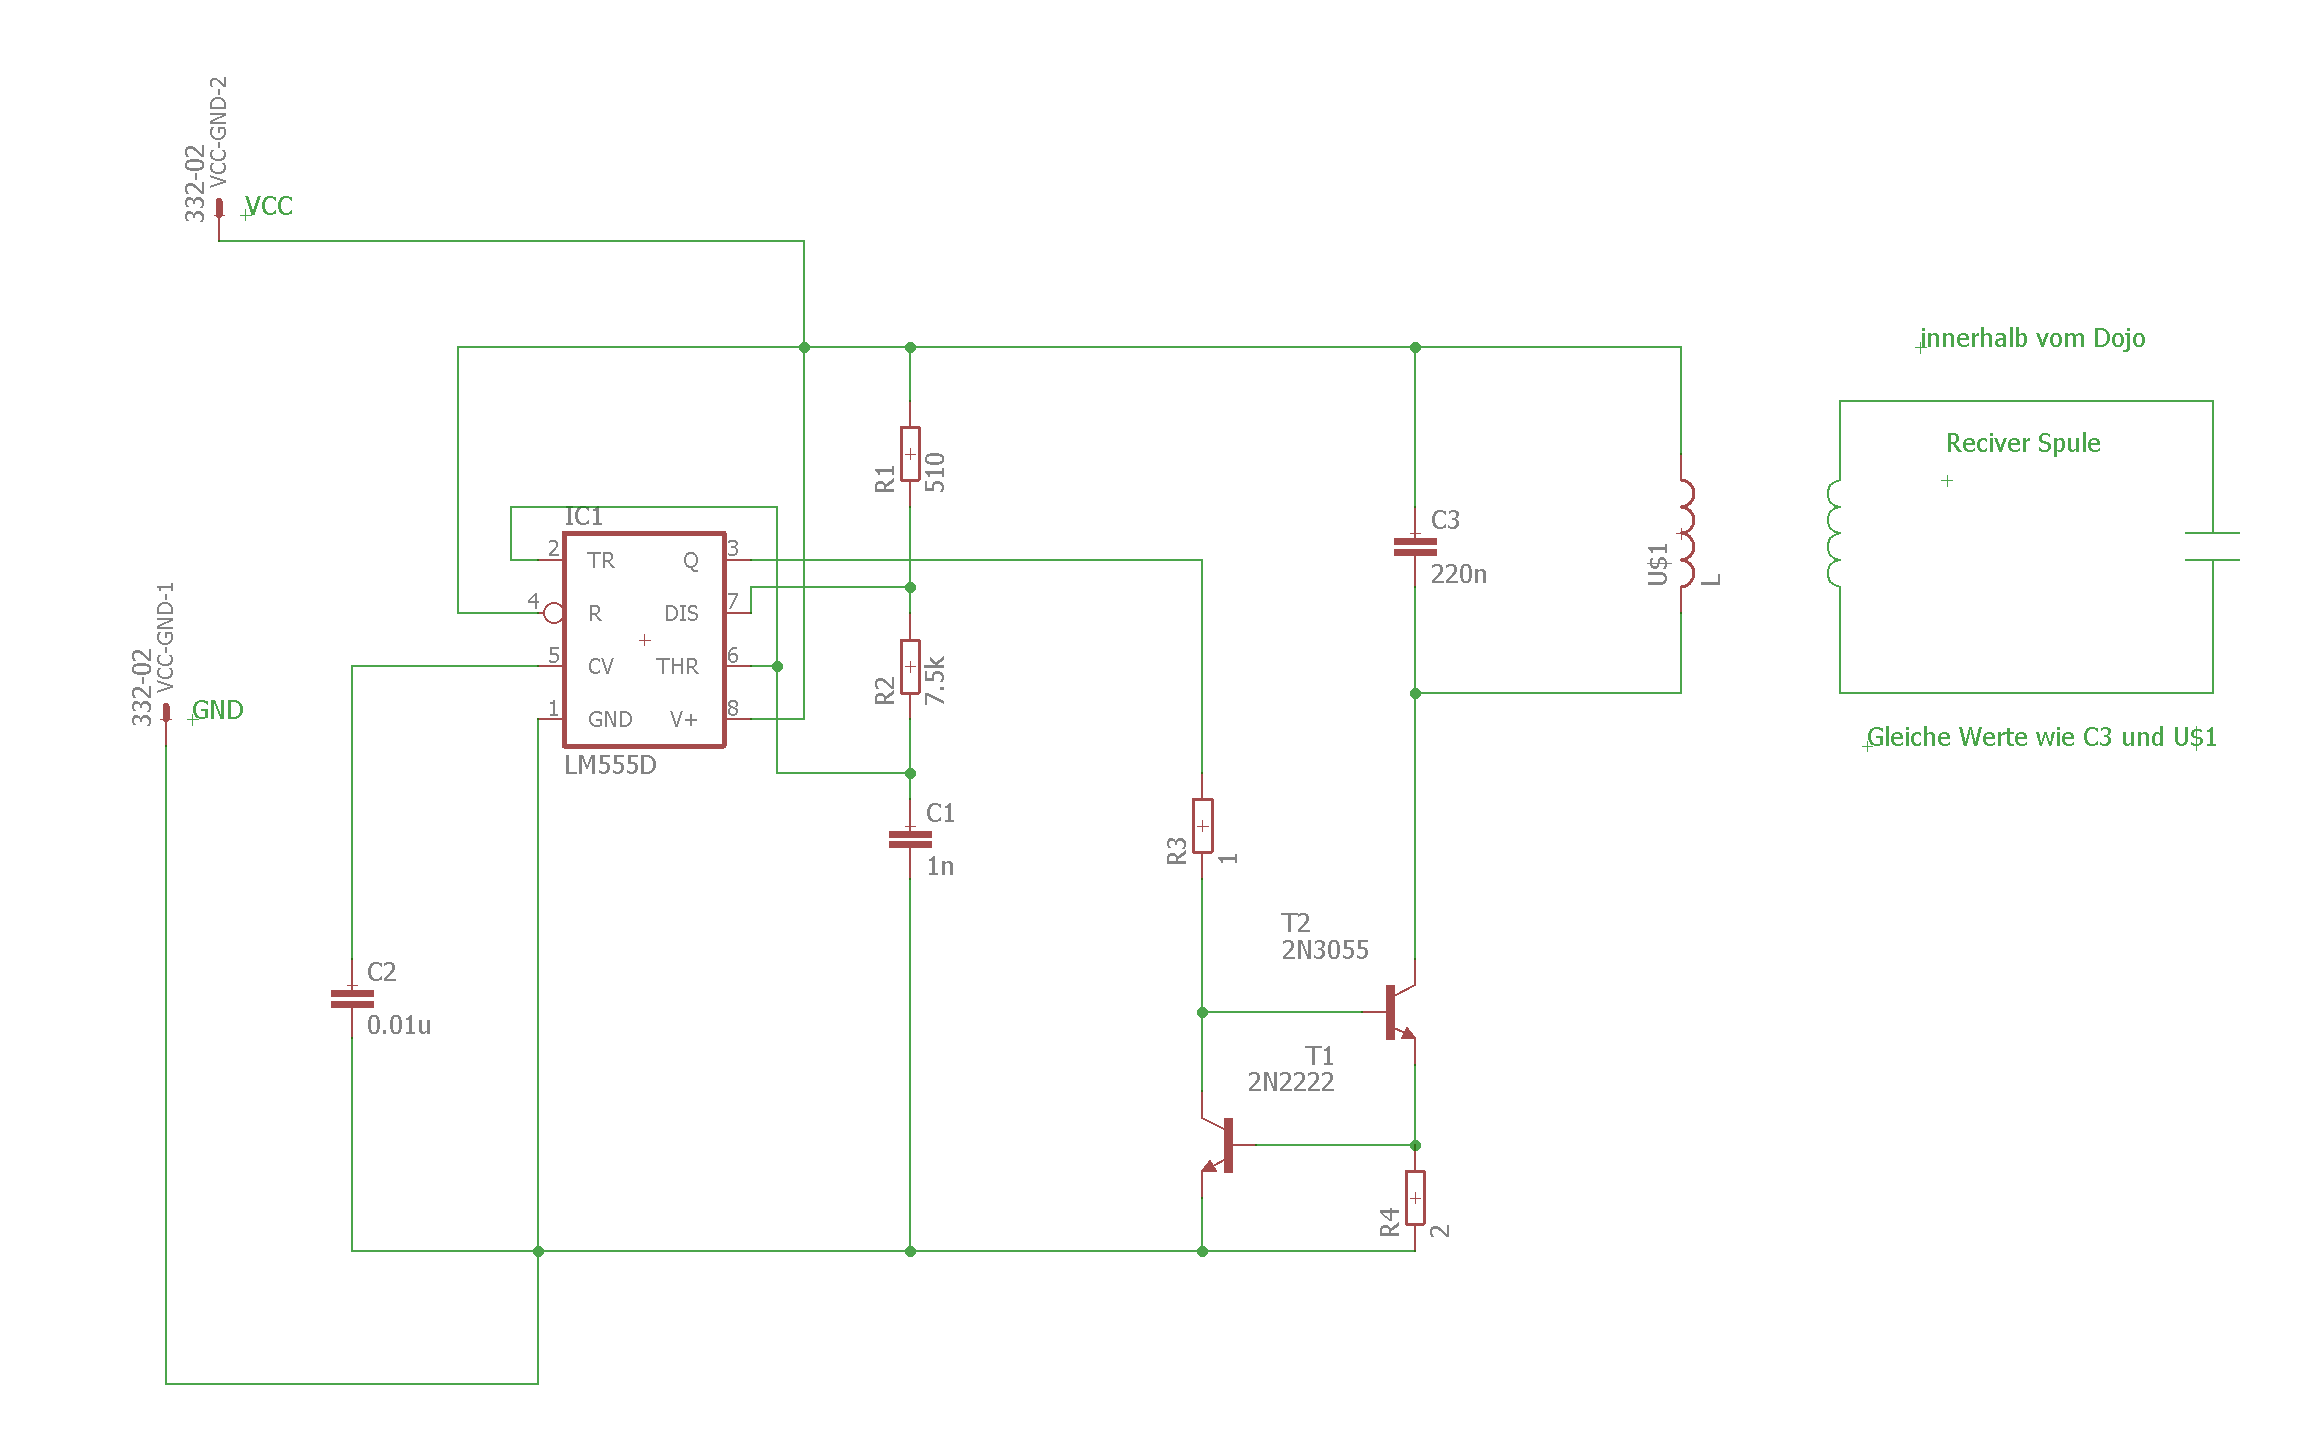
\includegraphics[width=\textwidth]{data/Tranceiver.png}
		\caption[Ne555]{Die verwendete Timerschaltung als Pulsquelle} %picture caption
		\label{fig:Tranceiver-Schaltung}
	\end{center}
\end{figure}
 
Das Pulssignal selber muss verschiedene Kriterien erfüllen. Zum einen sollte der Duty Cycle so nahe wie möglich an $50\%$ sein. Um dies zu erreichen muss $R2 >> R1$ gelten. Das andere Kriterium ist die Erreichung der Resonanzfrequenz des LC-Gliedes.Diese wird wie folgt aus den Komponenten des LC-Gliedes berechnet.

\begin{equation}\label{eq:Resonanz}
Resonanzfrequenz=1/2pi*sqrt(L*C)
\end{equation}

Die ideale Frequenz würde $93kHz$ betragen. Jedoch musste diese auf $79kHz$ angepasst werden da die nachfolgende Ladeschaltung nicht ideal dimensioniert wurde. Genaueres dazu ist in der Validierung der Hardware zu finden.
Um das Pulssignal theoretisch optimal einzustellen, können folgende Richtlinien betrachtet werden:
\begin{description}
	\item [$\cdot$ C] beeinflusst die Zeiten (Frequenz/High-Time/Low-Time)
	\item [$\cdot$ R$_{1}$] beeinflusst die High-Time, lässt jedoch die Low-Time unverändert.
	\item [$\cdot$ R$_{2}$ ] beeinflusst die High- und Low-Time und beeinflusst somit den Duty Cycle.
\end{description}


Die verwendeten Komponenten $C$, $R_{1}$ und $R_{2}$, welche in der Abbildung  \ref{fig:Tranceiver-Schaltung} rechts vom Timer Baustein zu sehen sind, wurden durch nachfolgende Formeln \ref{eq:TimerF} bis \ref{eq:TimerR2} berechnet. 


\begin{equation}\label{eq:Timerf}
f= \dfrac{1}{T}= \dfrac{1.44}{((R_{1} + 2 \cdot R_{2})\cdot C)}
\end{equation}
\begin{equation}\label{eq:TimerTL}
LowTime= 0.693 \cdot R \cdot C
\end{equation}
\begin{equation}\label{eq:TimerTH}
HighTime= 0.693 \cdot (R_{1} + R_{2}) \cdot C
\end{equation}
\begin{equation}\label{eq:TimerDC}
D = DutyCycle = \dfrac{R_{1} + R_{2}}{R_{1} + 2 \cdot R_{2}}
\end{equation}
\begin{equation}\label{eq:TimerR1}
R1 = 1.44 \cdot \left( \dfrac{2 \cdot D - 1}{f \cdot C} \right)
\end{equation}
\begin{equation}\label{eq:TimerR2}
R2 = 1.44 \cdot \left( \dfrac{1-D}{f \cdot C} \right)
\end{equation} 


Für die Berechnung der effektiven Werte, müssen die esten Werte angenommen werden. Deshalb lohnt es sich z.B. einen Wert für den Kondensator C anzunehmen, da dessen verfügbare Werte  durch die E-Reihen begrenzt sind. Es ist zu erwähnen, dass es sich bei den bereits eingefügten Zahlenwerten um Konstanten handelt, welche in jedem handelsüblichen Datenblatt eines $555$ Timer-Bausteins zu finden sind. Unsere Berechnungen ergaben folgende Werte für die angepasste Tranceiver Schaltung, welche mit der verringerten Taktfrequenz von $79.12 kHz$ betrieben wird.:

\begin{center}
C = $1nF$\\
R1 = $200\Omega$\\
R2 = $9k\Omega$\\
\end{center}

Zu sehen in Abbildung \ref{fig:Tranceiver-Schaltung}

Für die Berechnung der effektiven Werte, müssen die ersten Werte angenommen werden. Deshalb lohnt es sich z.B. einen Wert für den Kondensator C anzunehmen, da dessen verfügbare Werte durch die E-Reihen begrenzt sind. Es ist zu erwähnen, dass es sich bei den bereits eingefügten Zahlenwerten um Konstanten handelt, welche in jedem handelsüblichen Datenblatt eines $555$ Timer-Bausteins zu finden sind. Unsere Berechnungen ergaben folgende Werte für die angepasste Tranceiver Schaltung, welche mit der verringerten Taktfrequenz von $79.12 kHz$ betrieben wird.:

\begin{itemize}
\item C = $1nF$
\item R1 = $200\Omega$
\item R2 = $9k\Omega$
\end{itemize}
>>>>>>> bb39de6a20b2fac89fed3a9f18adab8773cde896
 
Gemäss Berechnung \ref{eq:Timerf} beträgt die Frequenz $79.12kHz$. Nach der Berechnung der Frequenz, können nun die einzelnen Komponenten ausgewählt und implementiert werden. Dabei gilt es zu beachten, dass minimale Abweichungen bereits zu einer Änderung der Frequenz, Pulsdauer und Duty-Cycle des Pulssignales führen.

\subsubsection*{Receiver}
<<<<<<< HEAD
Der Receiver besteht primär aus einem LC-Glied und einem Gleichrichter. Speziell ist, dass bei der Tranceiverschaltung das selbe LC-Glied verwendet wurde wie bei der Receiverschaltung. (Wie in Abbildung \ref{fig:Tranceiver-Schaltung} rechts oben zu sehen besteht das LC-Glied aus unserer Flachspule L mit einem Wert von $14.9uH$ und unserem Koppelkondensator C mit $220nF$)  Dies aus dem Grund, weil das Energiefeld bei einem identischen LC-Glieder Paar am effektivsten ausgenutzt werden kann. Das L-Glied (Flachspule) lässt sich mit einer Dimension von $\o 15mm$ Durchmesser und $0.2mm$ Höhe gut im inneren des Dōjō’s platzieren. Die Positionierung findet am Boden statt, da dieser eben ist und somit als Standfläche für den Dōjō genutzt wird. Somit kann dieser schlussendlich in der Ladesatation platziert werden, ohne dass Dieser gefahr läuft davon zu rollen. Die hochfrequente Wechselspannung welche nun gemessen werden kann, muss für die Speisung der Batterie noch gleichgerichtet werden. Hierbei können beliebige Dioden verwendet  und zu einem Brückengleichrichter verschaltet werden. Wir entschieden uns für Schotky-Dioden, da diese mit ihrer geringen Durchlassspannung von $0.2V$ die übertragene Spannung nur leicht abschwächen. Anschliessend wird die gesamte Ladeschaltung gespiesen, welche den gesamten Ladeprozess des Akkus übernimmt. Einen Einblick in diesen Ladeprozess gibt nachfolgendes Kapitel.

